\documentclass{article}
\usepackage[pdfborder={0 0 0}, colorlinks=true]{hyperref}
\usepackage{multicol}
\usepackage{color}
\usepackage[pdftex]{graphicx}
\author{CISC475/675 Spring 2010}

\title{REX User's Manual}
\date{\today}

\begin{document}

\maketitle
\begin{center}
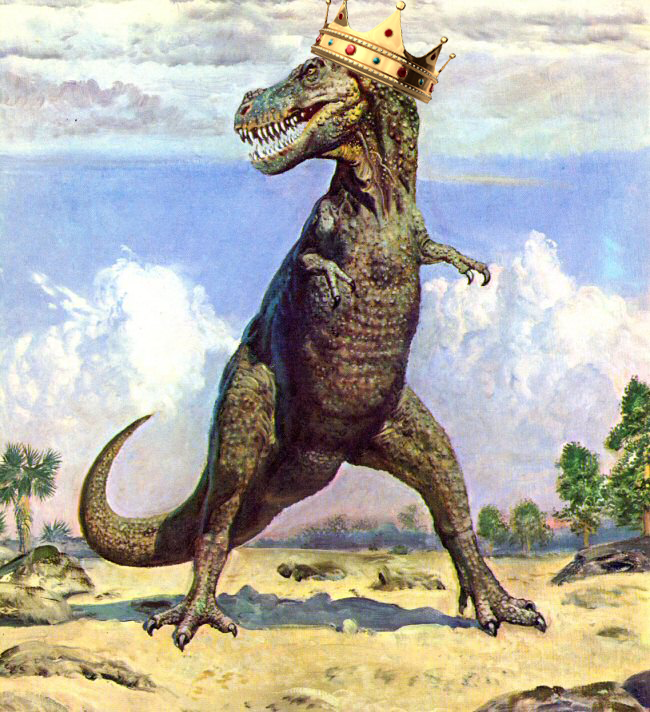
\includegraphics{rex.png}
\end{center}

\newpage
\tableofcontents
\newpage

\section{Introduction}
The REX software package assists in the creation of multiple choice exams.
It is advantageous to create multiple versions of the same exam with varied
questions to discourage cheating in packed lecture halls. This requires choosing
questions, rearranging their order, and reordering their answer for several
exams. The REX software reduces the effort required in this tedious process by automating the question selection and randomization process.

The REX software is cross-platform, open-source, and extendable. Standard 
\LaTeX{} format is used for the questions and output exams to enable hand editing
of exams. Every exam is supplied with an answer key for easy grading.

The program was created as a class project by the University of Delaware's 
Spring 2010 Advanced Software Engineering (CISC475/CISC675) class.  

\section{Overview}
The REX software package takes two input files: the Exam Configuration File
(ECF) specifies the composition of each exam, and the Universal Exam File
(UEF) contains the question bank. From these inputs multiple versions of the
exam are created. 

The order of sections, questions, and answers are all randomized differently on each version. There is the capacity to add figures, blocks of text, and an introduction (Referred to as front matter) to the exam. 


\section{Installation}
The REX software is contained in a single Java .jar file and has no
dependencies. No unpacking or installation is required, just locate the
\texttt{REX.jar} executable in the desired directory. Currently the program
only accepts command line input so UNIX systems are preferable. 

REX requires a Java 1.6 compatible JRE. 

\subsection{Building From Source}
Optionally the user can build REX from source if custom changes are made. 
\begin{itemize}
\item Install Ant and a Java 1.6 JDK
\item Checkout the project source code from the repository
\begin{verbatim}
svn co svn+ssh://[user]@cisc475.acad.cis.udel.edu/
home/www/repos/cisc475/trunk
\end{verbatim}
\item Download and extract necessary libraries (Antlr, Corbertura, and JUnit) to
trunk/lib from the following URI
\begin{verbatim}
http://eecis.udel.edu/~cates/rex-external-libs.tar.gz
\end{verbatim}
\item Create a build.properties file for your local machine in the root of trunk
\begin{verbatim}
cobertura.lib.dir=lib/cobertura-1.9.4.1
antlr3.name=lib/antlr-3.2.jar
antlr3-task.name=lib/antlr3-task.jar
junit.name=lib/junit-4.8.1.jar
\end{verbatim}
\item Run ant
\item Use java -jar REX.jar to execute the application
\end{itemize}


\section{Universal Exam File (UEF)}
The Universal Exam File stores all questions, answers, and figures that will be
included in the exam. REX can take a subsection of these questions as specified
in the Exam Configuration File. 

A UEF file is made up by a combination of problems, blocks and figures.

Please see Figure \ref{fig:SampleUEF} on page \pageref{fig:SampleUEF} for 
a complete Universal Exam File example.

\subsection{Frontmatter}
The Frontmatter is the introduction to the exam, all the content that appears before the first question, block or figure is defined. It is preserved verbatim in the generated exams, and aside from REX commands, any \LaTeX command may appear within the Frontmatter.

\subsection{Problems}
Problems are the heart and soul of a REX-generated exam. REX is built around a desire to select and randomize a set of problems, and Problems located in the UEF is how REX finds them.

Problems are defined by a \textbackslash{begin}[\textcolor{blue}{string required}]\{problem\}\{\textcolor{blue}{string topic}\}\\*\{\textcolor{blue}{decimal difficulty}\} command, which takes two mandatory arguments. The first is a topic argument. All problems of the same topic are automatically grouped together, although their order within the topic is random, and the order of the topics itself is also random. Topics are how you choose a problem using a \hyperref[GroupConstraints]{Group Constraint}. The second argument is the difficulty. This is a decimal value, either negative or positive, that is also used by Group Constraints to select and value problems.

The optional argument for Problems, \textcolor{blue}{string required}, is a string for the label of a block that is required by the problem. This will ensure that the referred block will always precede the problem.

The question (That is, prompt) for the problem is the text in the problem definition that is placed before the answers. Like the Frontmatter, the question can contain any \LaTeX command that is not also a REX command.

The problem definiton consists of everything between the \textbackslash{begin}\{problem\} and the \textbackslash{end}\{problem\}. Inside of there, you can either give the problem a label, or provide the answers for the problem.

\subsubsection{Problem Labels}
For problems, a label is optional. Labels are used to refer to a specific problem, and so, if you don't want to refer to the problem (Most likely through a \hyperref[RequiredProblemConstraints]{Required Problem Constraint}), it can be safely ommited.

To give a problem a label, you place a \textbackslash{label}\{\textcolor{blue}{string label}\} somewhere inside the problem definition.

\subsubsection{Problem Answers}
The answers inside a problem are grouped together by an ``answers environment'', that is, between a \textbackslash{begin}\{answers\} and a \textbackslash{end}\{answers\} \LaTeX command. A problem does not need to have an answers environment... it's perfectly acceptable to not have one, such as with a short answer or essay response question. However, if a problem does have an answers environment, it must contain at least one answer. Additionally, no problem may have more than 26 answers.

Each answer is defined by \textbackslash{answer}[\textcolor{blue}{optional correct}, \textcolor{blue}{optional fixed}]. As you might expect, the \textcolor{blue}{optional correct} defines whether the answer is a correct answer. REX uses the presence of the string \texttt{correct} in a pair of braces to determine if the answer should be considered correct, and the absence to indicate it should be considered incorrect. Similarly, the \textcolor{blue}{optional fixed} indicates whether the answer should be kept in its current location in the list of answers (Such as a ``None of the above'' response, which should always be last). Like with the \textcolor{blue}{optional correct} keyword, the \textcolor{blue}{optional fixed} keyword is used by determining the presence of the string \texttt{fixed} in a pair of braces in the answer definition.

If we wish to mark an answer as both correct and fixed, we would place them both in a single pair of braces, separated by a comma, as \texttt{[fixed, correct]} or \texttt{[correct, fixed]}

At least one answer must be labeled as correct, but it is acceptable to have more than one correct answer.

\subsubsection{Problem References}
A reference is similar to the required argument in the Problem definition. It is of the form \textbackslash{ref}\{\textcolor{blue}{string label}\}. This is most commonly used to refer to figures, as the required argument is used to refer to blocks. Like the required argument, the \textcolor{blue}{string label} points to the label of the figure you'd like to refer to, and all figures refered to this way will be placed before the problem in the output exam.

\subsubsection{Example Problem}
\begin{verbatim}
\begin{problem}[require=block topic]{Arithmetic}{5}
  \label{prob:arithmetic:prime}
  Which of the following is not prime?
  \ref{fig:figure topic}
  \begin{answers}
    \answer[correct] $2^{-1}$
    \answer[correct, fixed] $2^0$
    \answer $2^1$
    \answer $3^1$
    \answer[fixed] none of the above
  \end{answers}
\end{problem}
\end{verbatim}


\subsection{Blocks}
A block is any kind of non-floating latex text that is not part of a problem but might still be included in the exam after the front-matter, between the problems, or at the end of the exam after all problems. A typical case is text that is to be shared by several problems or some text at the end of the exam.

A block is inserted in a ``block'' environment. This takes one argument, which is just the label to give to the block. That is, it can be defined by \textbackslash{begin}\{block\}\{\textcolor{blue}{string label}\}.

\subsection{Figures}
%TODO
These are floating environments expressed in the usual \LaTeX way, using the figure environment. They can be labeled in the same way you would label a problem. A problem refers to a figure if a \textbackslash{ref} to the figure's label occurs anywhere in that problem's environment. If at least one problem referring to a figure A is included in a generated exam, the figure will also be included automatically. Every attempt will be made to include the figure before any of its associated problems, and, if possible, on the same page as the associated problems.

% How do we add color to this to make it easier
% to read? -Haley

% We can add color by using \textcolor{declared-color}{text} - BUT, we can't put that in a verbatim.
% We'd have to escape all the LaTeX commands to use that. We'd have to at the least place a 
% \textbackslash for ever instance of a backslash - \begin, \section, etc.
% Also, I can't find an easy way to make a long section of text appear teletype other than
% using \begin{verbatim}.
%\newpage

\begin{figure}[H]
%\subsection{Sample UEF File}
\begin{verbatim}
    \documentclass{exam} 
    \usepackage{fullpage}
    \usepackage{amsmath}
    \usepackage{comment}
    \usepackage{graphicx}

    \begin{document}

    \examheader{CISC 106}{UEF Example}{Developed: 2010}

    \section{Topic}

    \begin{block}{FSA Description}
      In the following four problems, let $A$ denote a finite-state
      automaton with exactly one accepting state.
    \end{block}

    \begin{problem}{topic}{15}
      This is a problem
      \begin{answers}
        \answer This is an answer that is not correct
        \answer answer
        \answer[fixed] This is a fixed answer that is not correct
        \answer[correct] This is a correct answer
        \answer answer
        \answer[fixed,correct] fixed correct answer
      \end{answers}
    \end{problem}

    \begin{figure}[placement h]
      \begin{center}
          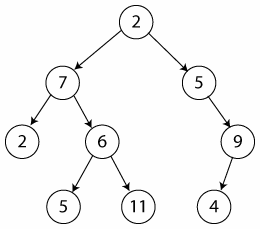
\includegraphics[scale=0.50]{binary_tree.png}
          \caption{Traverse Binary Tree}
          \label{fig:binary tree}
      \end{center}
    \end{figure}

    \begin{block}{Goodbye Message}
      Did you remember to write your name on the first page?
      Did you attempt to answer every question?
      Have a good holiday.
    \end{block}

    \end{document}
\end{verbatim}
\caption{Sample UEF.txt}
\label{fig:SampleUEF}
\end{figure}

%\newpage

\section{Exam Configuration File (ECF)}
The Exam Configuration File is a text file with a \texttt{.tex} extension
that consists of a series of constraints. Each constraint is separated by a semicolon,
with comments being all text that follows after a pound symbol 
(\texttt{\#}) until the end of the line. Please see section \ref{sec:exampleecf} for a complete example.

There are four defined commands for the ECF file.

\subsection{Group Constraints}
\label{GroupConstraints}
A group constraint is a command of the form \texttt{include \textcolor{blue}{int count}
problems on "\textcolor{blue}{string topic}" with difficulty in \textcolor{blue}{interval\footnote{An interval is a pair of decimals separated by two periods, in between a pair of braces or parenthesis. A brace on an end indicates that edge is inclusive, and a parenthesis that the edge is exclusive. For example, \texttt{[3..5)} would be the range from 3 to 5, including 3 but not including 5.} difficulty} at \textcolor{blue}{int \\* points} points;}.

The command will choose \textcolor{blue}{count} problems from \textcolor{blue}{topic} that fall in the \textcolor{blue}{difficulty} range, and assigns all of them \textcolor{blue}{points} points.

For overlapping constraints, REX will attempt find the largest set of questions that resolves all constraints. That is, if there exist two identical constraints for 5 problems each, REX will attempt to find 10 questions total. If REX cannot accomplish this, the request will result in an \hyperref[RexUnsatisfiableException]{RexUnsatisfiableException}. 

\subsection{Required Problem Constraints}
\label{RequiredProblemConstraints}
A required problem constraint is a command of the form \texttt{includeall "\textcolor{blue}{string label}" at \textcolor{blue}{int points} points;}.

This will ensure the the question with the \textcolor{blue}{label} given is included in every
generated exam, and will be given \textcolor{blue}{points} points. 

Multiple \textcolor{blue}{label}'s can be given in one command by separating them by commas. This will have the same effect as if each label was given on its own line.

\subsection{Append Text}
An append text command is a command of the form \texttt{append "\textcolor{blue}{string label}";}

This will take the text contained in the block with the given \textcolor{blue}{label}, and append it to the end of the exam.

\subsection{Version Definition}
A version definition of a command of the form \texttt{versions are "\textcolor{blue}{string\\ versions}";}

\textcolor{blue}{Versions} are a list of strings, separated by commas, used to distinguish the different exams generated. Each generated exam will use one item in the list, and so there must be at least as many items as there will be exams generated. 

In the UEF file, you can use the \textbackslash{examversion} command to insert the current version string. One example use for this is to have a different date format for each generated exam, so that the exams can be easily distinguished from one another, but a naive student would not know how to tell if his neighbor has a similar exam.

\subsection{Example ECF}
\label{sec:exampleecf}
\begin{verbatim}
include 5 problems on "Finite State Automata" with difficulty 
  in [0,20) at 3 points;
include 5 problems on "ssort" with difficulty in [20,\infty) at 
  2 points;
include 3 problems on "arithmetic" with difficulty in [0,10] at 
  1 points;
include 3 problems on "arithmetic" with difficulty in 
  (-\infty,\infty) at 3 points;

# the following problems will be included in their 
# corresponding sections on any generated exam
includeall prob:arithmetic:prime, prob:arithmetic:composite, 
  prob:misc:hat,prob:misc:complexity at 5 points;

append "Goodbye Message"; # this block will be added at end

versions are "1/21/2010", "Jan.\ 21, 2010", "21-jan-2010", 
  "JAN.\ 21 2010";
\end{verbatim}

\section{Usage}
\begin{verbatim}
java -jar REX.jar 
Usage: rex [options] <UEF filename> <ECF filename>
Options: 
    -n numExams : int numExams declares number of exams
    -seed seed : long seed declaresthe seed for randomization
    -pdf       : .tex files are automatically converted to PDF
\end{verbatim}

\subsection{Synopsis}
java -jar REX.jar [-n numExams] [-seed seed] [-pdf] UEF-file ECF-file

\subsection{Description}
REX will parse through the UEF and ECF files and generate the appropriate number
of output exams, as specified in the ECF file or on the command line.

\noindent Below are the options:\\
\indent \textbf{-n numExams} will generate \textbf{numExams} different exams\\
\indent \textbf{-seed seed} will generate the exams based on the specific \textbf{seed}\\
\indent \textbf{-pdf} will create a PDF file from the generatex \LaTeX{} files\\

\noindent \textbf{NOTE:} The PDF option requires a \LaTeX{} interpreter to be installed. See next section.

\subsection{Using the PDF option}
In order for the exams to be output in a pdf format the file \verb|"Exam.cls"| must
be in the location from which the java -jar REX command is being run. If this file is not given
and the -pdf option is used an error such as the one below will display on the command line.
If the file is accidentally deleted copy from below
\\
\verb|pdflatex found error: "! LaTeX Error: Environment block undefined."|

\section{Troubleshooting}
Because of the requirements that REX places upon the input it parses, REX may present the user with a variety of errors. Additionally, it's possible that REX might process the request without any errors or warnings, but will provide an undesired output.

\subsection{Errors}

\subsubsection{RexException}
This error is thrown if there are problems throughout the REX process.
The exception is thrown with a useful error message.

\subsubsection{RexParseException}
This error means that REX encountered a syntactic error in either the UEF or ECF file. Please consult the provided error message for more information.

\subsubsection{RexUnsatisfiableException}
\label{RexUnsatisfiableException}
This error means that the input files were parsed correctly, but that
REX determined that the requirements from the ECF cannot be resolved
using the provided UEF file. Generally, this means that there aren't
enough problems in the UEF. Either reduce the number of requested
problems in the ECF, or create new problems in the UEF to resolve
this error.

Note: REX resolves the requirements in the ECF simultaneously. This means
that if the ECF has two identical requirements of 5 questions each, REX
will require at least 10 satisfactory questions.






\newpage
\section{Credit/Copyright}
\begin{itemize}
\item Prof Stephen Siegel (instructor) - siegel
\item Charlie Greenbacker (TA) - charlieg
\item Aaron Landwehr - alandweh
\item Ahmed El-Hassany - elhassa
\item Anthony Platt - aplatt
\item Burke Cates - cates
\item Fran ``Da Man'' Fitzpatrick - fitzpatr
\item Greg Simons - simons
\item Haley Boyd - boyd
\item Ian Burns - iburns
\item Jack Song - jsong
\item James Cardona - cardona
\item Jeremy Verchick - verchick
\item Jesse Gledhill - gledhill
\item Josh Rothhaupt- rothhaup
\item Justin Johnson - justinjo
\item Keith McLoughlin - mcloughl
\item Kevin Schultz - schultz
\item Kyle Bouchard - bouchard
\item Lucero Carmona - carmona
\item Reed Martz - martz
\item Tim Armstrong - armstron
\item Tim McClory - tmcclory
\item Trevor Kiernan - kiernan
\item William Gordon - wgordon
\item Zach Hine - zhine
\end{itemize}

\newpage
\section{License}
\begin{verbatim}

Copyright (C) 2010  University of Delaware CISC475/675 Spring 2010 Class

This program is free software: you can redistribute it and/or modify
it under the terms of the GNU General Public License as published by
the Free Software Foundation, either version 3 of the License, or
(at your option) any later version.

This program is distributed in the hope that it will be useful,
but WITHOUT ANY WARRANTY; without even the implied warranty of
MERCHANTABILITY or FITNESS FOR A PARTICULAR PURPOSE.  See the
GNU General Public License for more details.

You should have received a copy of the GNU General Public License
along with this program.  If not, see <http://www.gnu.org/licenses/>.
\end{verbatim}

For more information on the GNU GPL, see \texttt{http://www.gnu.org/licenses/}.

\end{document}

